% !TEX root = paper.tex

\documentclass[11pt,letterpaper]{article}

% Packages
\usepackage{packages}
\addbibresource{sources.bib}

% Document Settings
\geometry{margin=1in}
\setlength{\parskip}{1ex}
\setlength{\parindent}{0pt}



\pagestyle{fancy}
\lhead{Väinö-verneri Kauppila} % controls the left corner of the header
\chead{} % controls the center of the header
\rhead{} % controls the right corner of the header
\lfoot{} % controls the left corner of the footer
\cfoot{} % controls the center of the footer
\rfoot{Page~\thepage} % controls the right corner of the footer
\renewcommand{\headrulewidth}{0.4pt}
\renewcommand{\footrulewidth}{0.4pt}

% =========================================
%             DOCUMENT
% =========================================

\begin{document}
%\doublespacing % Double spacing throughout the document


% =========================
%      TITLE PAGE
% =========================

% Suppresses headers, footers, and page numbers on title page
\begin{titlepage}
    \begin{center}
        \vspace*{4cm}
        Geography\\
        Internal Assessment \\
        \vspace{1cm}
        How does environmental quality, determined by the severity of pollution and the availability of green spaces, differ between a tourist-catering area of Paris versus a residential area? \\
        \vspace{1cm}
        \textit{Väinö-Verneri Kauppila} \\
        May 2021 \\
        \vspace{4cm}
        Word count: \textit{TBD} \\
        \vfill
        \vspace{0.1cm}
    \end{center}
\end{titlepage}

% =========================
%      DOCUMENT BODY
% =========================

\pagenumbering{roman}

\begin{center}
    \pdfbookmark{\contentsname}{Contents}
    \tableofcontents
    \vspace{1in}

\end{center}


% TODO: Add hyper-references to links
% TODO: Improve listings' styling
% TODO: Add links to Contents entries

\newpage

\pagenumbering{arabic}

\section{Introduction}

\subsection{Fieldwork question}

How does environmental quality, determined by the severity of pollution and the availability of green spaces, differ between a touristic area of Paris and a residential area?

In order to answer this question, the fieldwork for our paper was conducted in Paris, one of the largest and most well known cities in the world. The city itself is arranged into 20 districts, known locally as \textit{arrondissements}, are placed in a spiral in the city. It is globally known for its high number of tourists per year, equating to around 35 million in the year 2019 alone. \footcite{statista_department_27_2020} Many of them come to visit the world-renowned Eiffel Tower, located in the VII\textsuperscript{th} \textit{arrondissement}. \footcite{condor_ferries} To add, Paris is home to 2.2 million people, who mostly live in the outer residential areas, from the XI\textsuperscript{th} to the XX\textsuperscript{th} \textit{arrondissements}.

\begin{figure}[h!]
    \centering
    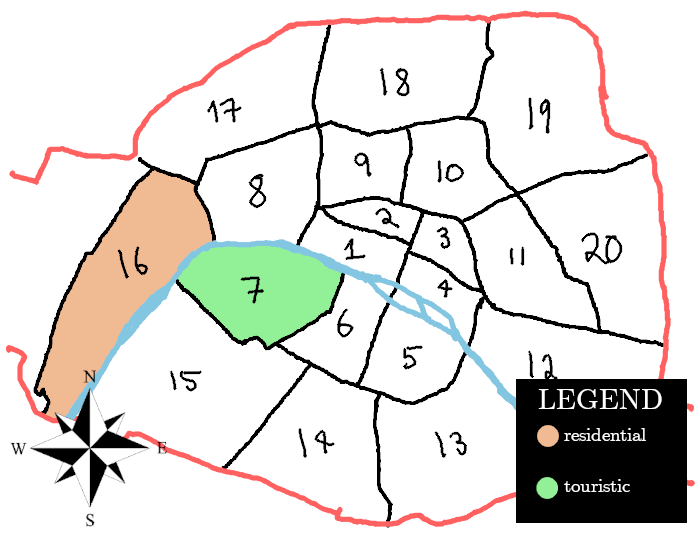
\includegraphics[width=0.7\linewidth]{media/arrts.png}
    \caption{A map of Paris \textit{arrondissements}, drawn by hand.}
\end{figure}



\subsection{Hypotheses}

\begin{enumerate}
    \item According to the Global Development Goals of the UN, 90\% of urban areas in the world had polluted air in 2016. \footcite{sdg_report_2020} Paris was among countries that didn't satisfy WHO's air quality minimum \footcite{ambient_outdoor_air_pollution_2018} of 2018, with on average a 50\% higher than normal pollution density. However, a counterargument to this could be that despite a higher concentration of people, tourist areas in Paris do not suffer as much from high traffic conditions from things such as typical morning rush hours, and tourists preferably using public transport or bikes.

    \item As there are more people moving about in residential areas, for example in cars for the morning commute or at noon for lunch, it can logically be theorized that noise pollution, which is obviously a function of the amount of cars, would be higher in these places. Today it is estimated that an average noise level of $60dB$ can be found in residential areas, according to the very comprehensive Bruitparif government-sponsored report. \footcite{bruitparif} This value largely surpasses the WHO's safe level of $53dB$. \footcite{who_noise_guidelines}

    \item The Parisian mayor, Anne Hidalgo included the improvement of environmental quality in her campaign. The mayor has promised to make so-called "green spaces" no further than 200 meters to any person,\footcite{anne_hidalgo_2020} and as such, it should be hypothesized that green spaces, which include parks, agglomerations of trees, shall be distributed evenly with no difference between residential and touristic areas. The mayor emphasized on "urban forests" --- places where residents and tourists alike could enjoy the company of trees while walking along the city streets.
\end{enumerate}


%\begin{figure}[h!]
%    \begin{minipage}{\textwidth}
%        \centering
%        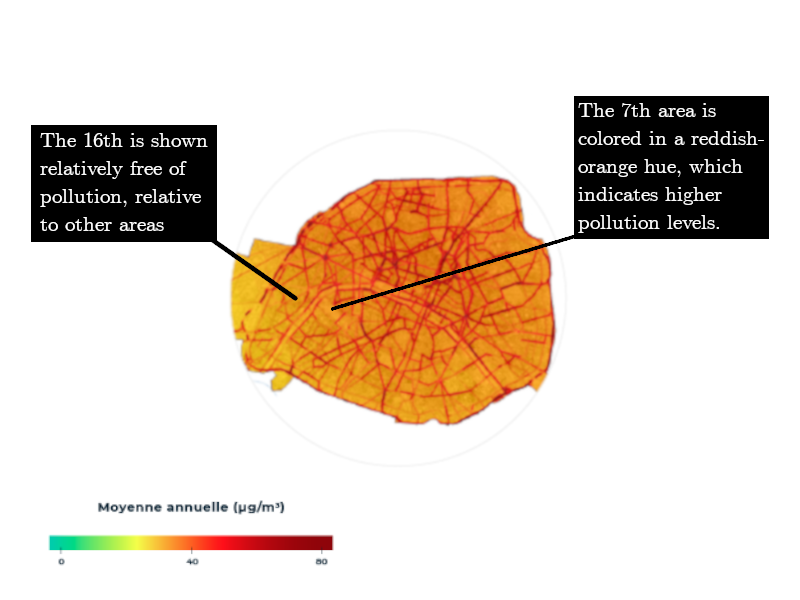
\includegraphics[width=0.7\linewidth]{media/no2_map.png}
%        \caption{A map of Paris NO2 levels in 2018, as reported by AirParif, on the official Paris website \protect\footcite{paris_air_qual}}
%    \end{minipage}
%\end{figure}

% NEW SECTION

\section{Method}


For our investigation, the topic in question is the environmental quality. We will compare the environmental quality of two areas, one meant as a residential one and one with a heavy tourist presence. To best represent these areas, we have chosen the XVIe and the VIIe. The XVIe is home to many housing complexes and fosters facilities aimed at catering to the residents whereas the VIIe sees many tourists as it is home to the famed Eiffel Tower and the Seine river, prime tourist attractions of Paris.

\subsection{Study site choices}

We chose 10 sites in total to conduct a bipolar survey, shown below in Figures 2, 3.

\begin{figure}[H]
    \begin{minipage}{\textwidth}
        \centering
        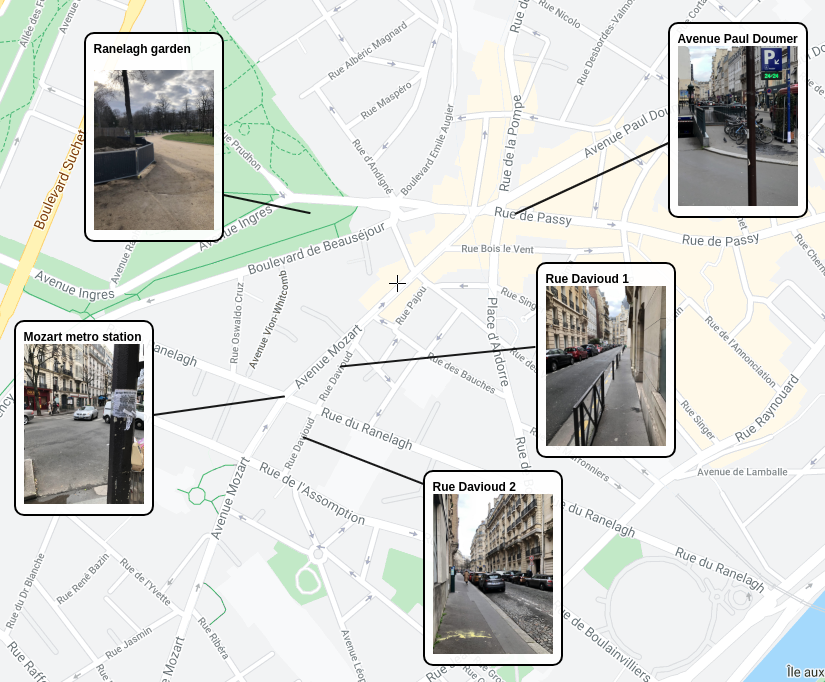
\includegraphics[width=0.7\linewidth]{media/16esites.png}
        \caption{Map of sites chosen for the residential area, the XVI\textsuperscript{th} \textit{arrondissement}. Map base layer courtesy of Google Maps, pictures seen are taken on a mobile phone.}
    \end{minipage}
\end{figure}

This site was chosen as, like stated before, it is a residential area. There are other residential areas in Paris, however this one was specifically chosen for reasons of convenience.

\begin{figure}[H]
    \begin{minipage}{\textwidth}
        \centering
        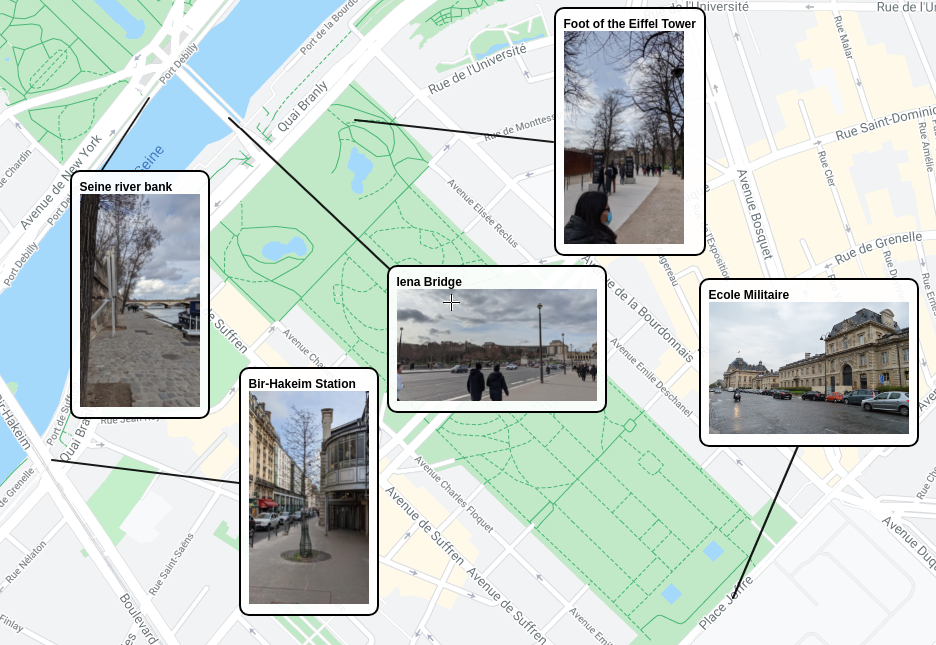
\includegraphics[width=0.7\linewidth]{media/7esites.png}
        \caption{Map of sites chosen for the residential area, the XVI\textsuperscript{th} \textit{arrondissement}. Map base layer courtesy of Google Maps, pictures seen are taken on a mobile phone.}
    \end{minipage}
\end{figure}

This area in the VII\textsuperscript{th} was chosen as it is a staple of tourism in France. It is home to the famed Eiffel Tower, the Ecole Militaire building and the Seine river bank.

\subsubsection{Our sampling method}

The sites in the two areas were chosen using a method of stratified sampling. Considering the VII\textsuperscript{th} does indeed contain residential sites and the XVI\textsuperscript{th} touristic ones, we can discard the ones that are irrelevant to our study.

\subsection{Method}

\subsubsection{Bipolar semantic survey}

The sites were visited to conduct a so-called "bipolar survey", which consisted of rating the site based on multiple criteria. This process was done by selecting a single person from our group to visit one of the sites, and complete a bipolar semantic survey. They would grade several different aspects of the site (such as general cleanliness, noise, amount of cars), and take a set of 3 images of the site.\footnote{Images taken for our study can be found at \url{https://github.com/kinnounko/notes/tree/main/geography/ia/images}} Our surveys were conducted during the week of the 10th of March, 2021 in the afternoon each time. The weather was overcast and moderately cold.

Our results for the bipolar survey are shown in Appendix \ref{app:bipolar}

When tallied, the total scores for each site can be expressed as a fraction over 84, as shown in Figures 4, 5.

\begin{figure}[H]
    \begin{center}
        \begin{tabular}{||c c||}
            \hline
            Site                     & Total score \\ [0.5ex]
            \hline\hline
            Bir-Hakeim               & 51          \\
            \hline
            Seine river bank         & 69          \\
            \hline
            Foot of the Eiffel Tower & 45          \\
            \hline
            Iena Bridge              & 42          \\
            \hline
            Ecole Militaire          & 54          \\ [1ex]
            \hline
        \end{tabular}
    \end{center}
    \caption{Total Bipolar Semantic scores for the VII\textsuperscript{th}}
\end{figure}

\begin{figure}[H]
    \begin{center}
        \begin{tabular}{||c c||}
            \hline
            Site               & Total score \\ [0.5ex]
            \hline\hline
            Rue Davioud 1      & 47          \\
            \hline
            Rue Davioud 2      & 53          \\
            \hline
            Avenue Mozart      & 31          \\
            \hline
            Avenue Paul Doumer & 35          \\
            \hline
            Ranelagh Garden    & 77          \\ [1ex]
            \hline
        \end{tabular}
    \end{center}
    \caption{Total Bipolar Semantic scores for the XVI\textsuperscript{th}}
\end{figure}

When plotted on a map, these totals can be shown with a gradient of colors.

\begin{figure}[H]
    \centering
    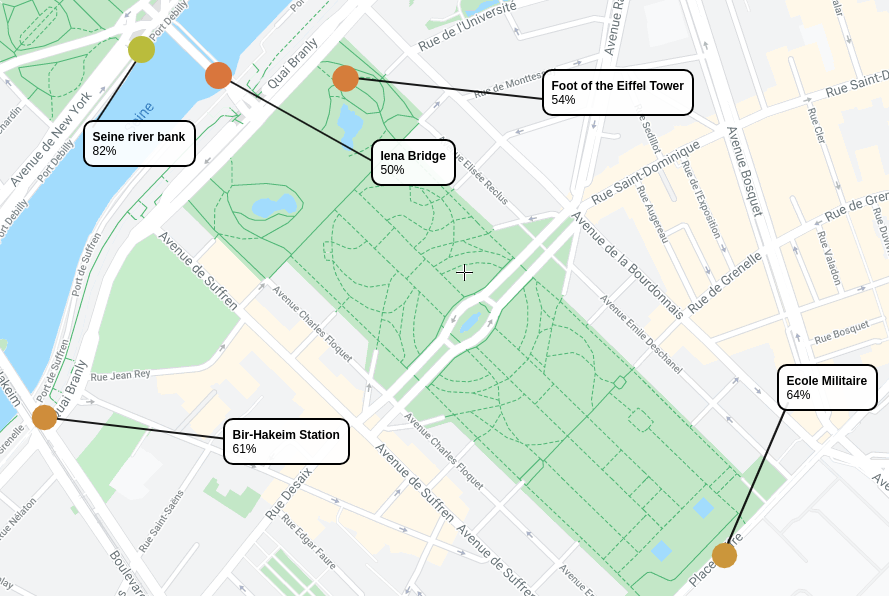
\includegraphics[width=0.7\linewidth]{media/7eColors.png}
    \caption{Each site in the VVI\textsuperscript{th}, with its respective total score expressed as a percentage for clarity, and a color assigned based on the gradient in Figure 8.}
\end{figure}

\begin{figure}[H]
    \centering
    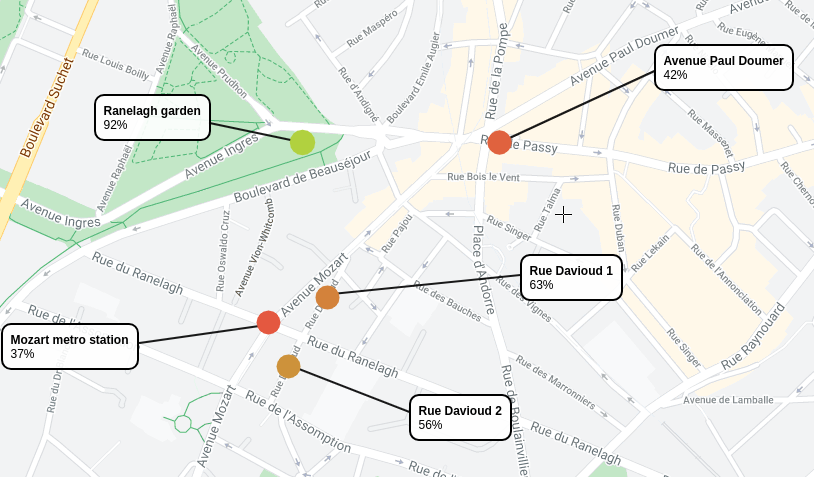
\includegraphics[width=0.7\linewidth]{media/16eColors.png}
    \caption{Each site in the XVI\textsuperscript{th}, with a percentage. Color assigned with gradient in Figure 8.}
\end{figure}


\begin{figure}[H]
    \centering
    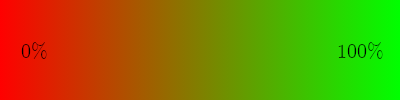
\includegraphics[width=0.4\linewidth]{media/bipolar/gradient.png}
    \caption{Gradient from red (hex color \#FF0000) for 0\%, to green (hex color \#00FF00) for 100\%. }
\end{figure}


\subsubsection{Statistical evaluations}

In order to either support or disprove our third hypothesis, it is important to study how trees are scattered in Paris, which reveals how dispersed green spaces are from one another. A statistical test called the Nearest Neighbor Index (NNI) test can provide a reasonable answer to this: if the index is similar for both sites, it can easily be said then that our hypothesis is supported. This value also reveals information about the distribution of trees: clustered, random or in a regular pattern, as seen in Figure 5 below.

\begin{figure}[H]
    \centering
    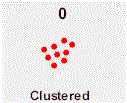
\includegraphics[width=0.2\linewidth]{media/nni1.png}
    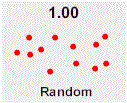
\includegraphics[width=0.2\linewidth]{media/nni2.png}
    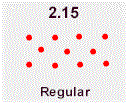
\includegraphics[width=0.2\linewidth]{media/nni3.png}
    \caption{The NNI measures the spacial distribution of data. From a value of 0, representing a clustered pattern, to 1 (random) and to 2.15 (uniform pattern)}
\end{figure}

As individually counting trees in these areas would be a tedious task, we used the Paris OpenData platform (licensed under the permissive ODbL license\footcite{odbl}), owned by the government. The fact that this kind of database platform exists, shows a certain level of transparency on the government's part.

We used the trees dataset procured from the library, which contains the exact coordinates of trees in the city. \footcite{paris_opendata} There are also other information such as species of the tree and such, however these are cleaned from the dataset for our purposes.

A script, written in Python was tasked to calculate the NNI value, because with a dataset of over 20,000 data points this would not be possible by hand. We go through each point, and find its nearest neighbor. In order to calculate distances between these two points, we use the Haversine Formula, as the two points would be in the form of coordinates. With this information the NNI can be calculated with the simple formula

$$Rn = \frac{2 \bar D}{\sqrt{\frac{a}{n}}}$$

where $Rn$ is the NNI index value, $\bar D$ is the mean observed distance to the nearest neighbor, $a$ is the area of the zone and $n$ is the total number of data points.



% NEW SECTION

\section{Analysis}

\textit{Not done}

\subsection{Environmental and cultural sustainability}
\textit{Not done}

\subsection{Economic sustainability}
\textit{Not done}

\section{Conclusion}

\textit{Not done}

\newpage
\pagenumbering{roman}


\section*{Notes}
\label{sec:notes}
\addcontentsline{toc}{section}{\nameref{sec:notes}}

This paper is written with the aid of the typesetting software \LaTeX. On a PDF viewer, the sections in the table of contents can be clicked to access that section.

All media and information related to this IA can be found on the URL \url{https://github.com/kinnounko/notes/tree/main/geography/ia}. This includes images, the \LaTeX{} source code to this paper, and the Python program used to calculate the NNI value.

\printbibliography

\appendix
\section{Appendix}
\label{app}

\subsection{Bipolar survey results}
\label{app:bipolar}

Shown below are our results from our bipolar semantic survey:

XVI\textsuperscript{th} residential area:

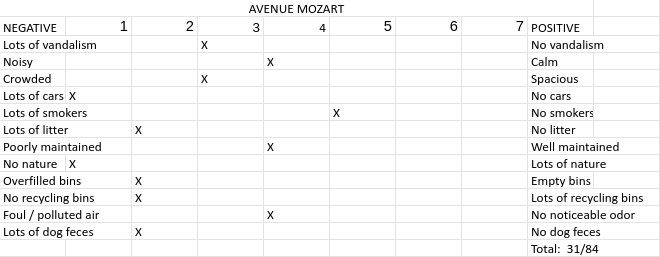
\includegraphics[width=0.5\linewidth]{media/bipolar/mozart.png}
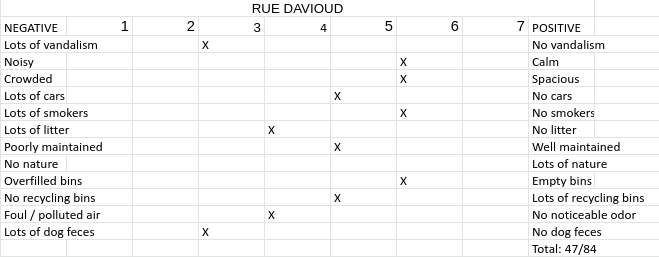
\includegraphics[width=0.5\linewidth]{media/bipolar/davioud1.png}
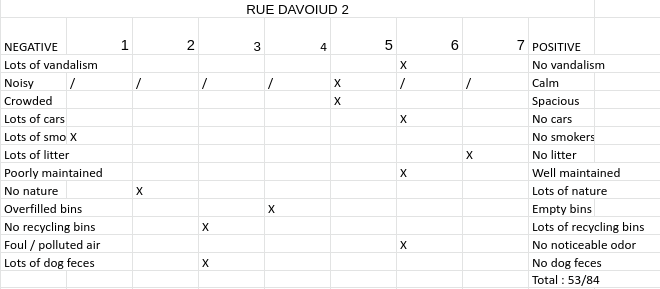
\includegraphics[width=0.5\linewidth]{media/bipolar/davioud2.png}
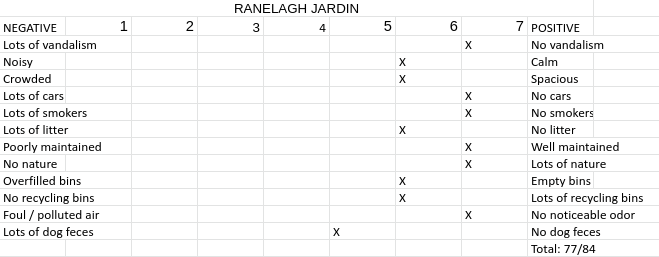
\includegraphics[width=0.5\linewidth]{media/bipolar/ranelagh.png}
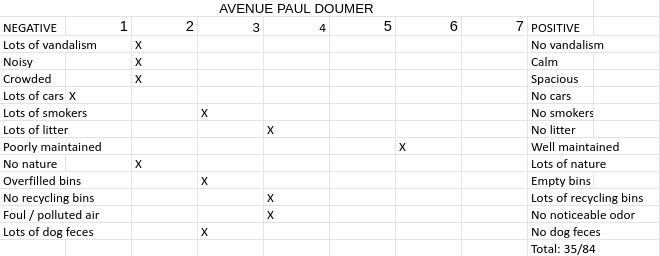
\includegraphics[width=0.5\linewidth]{media/bipolar/pauldoumer.png}

VII\textsuperscript{th} touristic area:

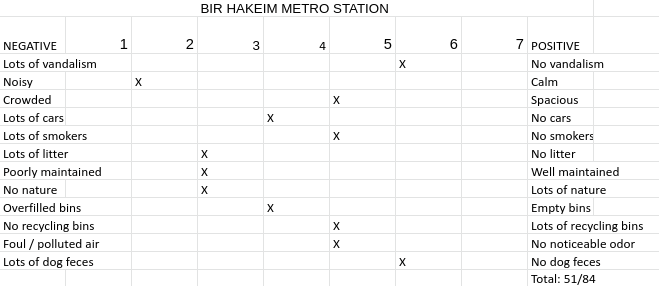
\includegraphics[width=0.5\linewidth]{media/bipolar/birhakeim.png}
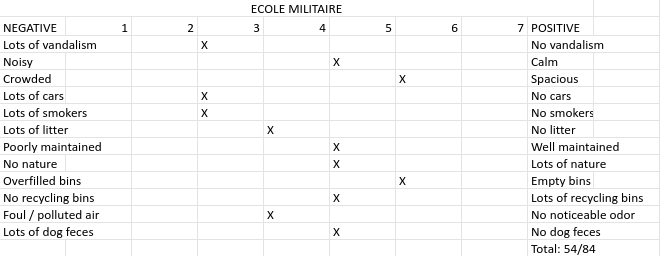
\includegraphics[width=0.5\linewidth]{media/bipolar/ecolemilitaire.png}
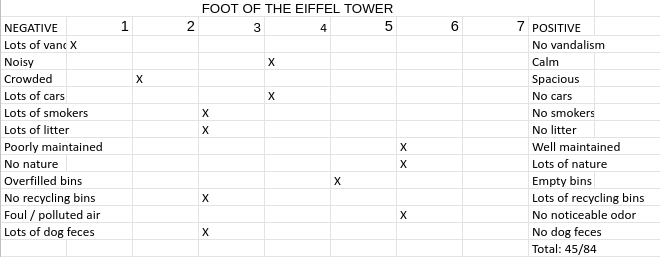
\includegraphics[width=0.5\linewidth]{media/bipolar/eiffel.png}
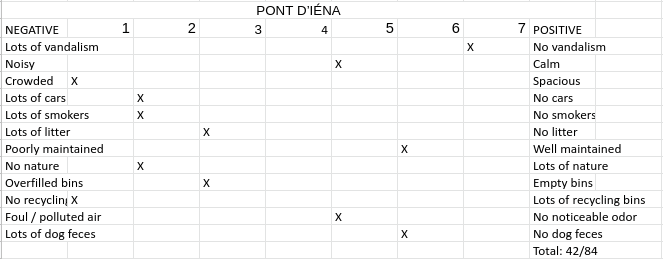
\includegraphics[width=0.5\linewidth]{media/bipolar/iena.png}
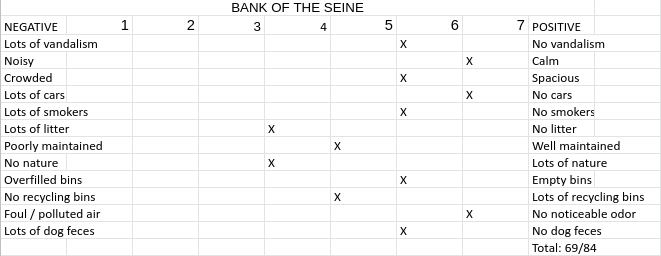
\includegraphics[width=0.5\linewidth]{media/bipolar/seinebank.png}

\end{document}